\documentclass{zjusct-beamer/zjusctbeamer}

% Metadata
\title{A First Look at the CPU Parallel Programming Framework}
\subtitle{PM - C++ Concurrency in Action}
\author[bowling233]{Baolin Zhu (@bowling233)}
\date{\today}
\institute[ZJUSCT]{Zhejiang University Supercomputing Team}
\copyleftnotice{CC-BY 4.0}

\hypersetup{
    pdftitle={\title},
    pdfpagemode=FullScreen,
}

\setminted{
    fontsize=\tiny % 设置代码和行号的字体大小
}

\begin{document}

% Set Mono and Emoji font
\setmonofont{DejaVu Sans Mono}
\setemojifont{TwemojiMozilla}

\maketitle

% Outline (Table of Contents)
\cutoc

% Slide 正文均使用英文
\section{Introduction}

% 我的简介
\begin{frame}[fragile]{\emoji{bust-in-silhouette} Biography}
	\begin{center}
		\begin{itemize}
			\item \textbf{Baolin Zhu} (\emoji{bowling} @bowling233)
			\item (with Eric) Leader of ZJUSCT
			\item \textbf{Research Interests}: Arch/OS, Three Pillars (Compute, Network and Storage)
		\end{itemize}
		\begin{tikzpicture}
			% Timeline base line
			\draw[thick, gray] (0,0) -- (10.5,0);

			% Node 0: CKC AGC
			\fill[blue] (1.5, 0) circle (0.1);
			\draw[gray] (1.5, 0) -- (1.5, 0.5);
			\node at (1.5, 1) {
\includegraphics[width=0.8cm]{day8_pm/img/bio-ckcagc.png}};
			\node[font=\bfseries\small] at (1.5, 2) {CKC AGC};
			\node[font=\footnotesize, gray] at (1.5, -0.5) {Freshman};

			% Node 1: ZJUSCT
			\fill[blue] (4.0, 0) circle (0.1);
			\draw[gray] (4.0, 0) -- (4, 0.5);
			\node at (4.0, 1) {
\includegraphics[width=0.8cm]{day8_pm/img/bio-zjusct.png}};
			\node[font=\bfseries\small] at (4.0, 2) {ZJUSCT};
			\node[font=\footnotesize, gray] at (4.0, -0.5) {Sophomore};

			% Node 2: RC4ML Lab
			\fill[blue] (6.5, 0) circle (0.1);
			\draw[gray] (6.5, 0) -- (6.5, 0.5);
			\node at (6.5, 1) {
\includegraphics[width=0.8cm]{day8_pm/img/bio-rc4ml.png}};
			\node[font=\bfseries\small] at (6.5, 2) {RC4ML Lab};
			\node[font=\footnotesize, gray] at (6.5, -0.5) {Junior};

			% Node 3: Tencent
			\fill[blue] (9.0, 0) circle (0.1);
			\draw[gray] (9.0, 0) -- (9.0, 0.5);
			\node at (9.0, 1) {
\includegraphics[width=0.8cm]{day8_pm/img/bio-csig.png}};
			\node[font=\bfseries\small] at (9.0, 2) {Tencent CSIG};
			\node[font=\footnotesize, gray] at (9.0, -0.5) {Junior};

		\end{tikzpicture}
	\end{center}
\end{frame}

% 本节课的参考教材
\begin{frame}[fragile]{\emoji{books} Textbook}

	\begin{columns}
		\begin{column}{0.4\textwidth}
			\begin{center}
				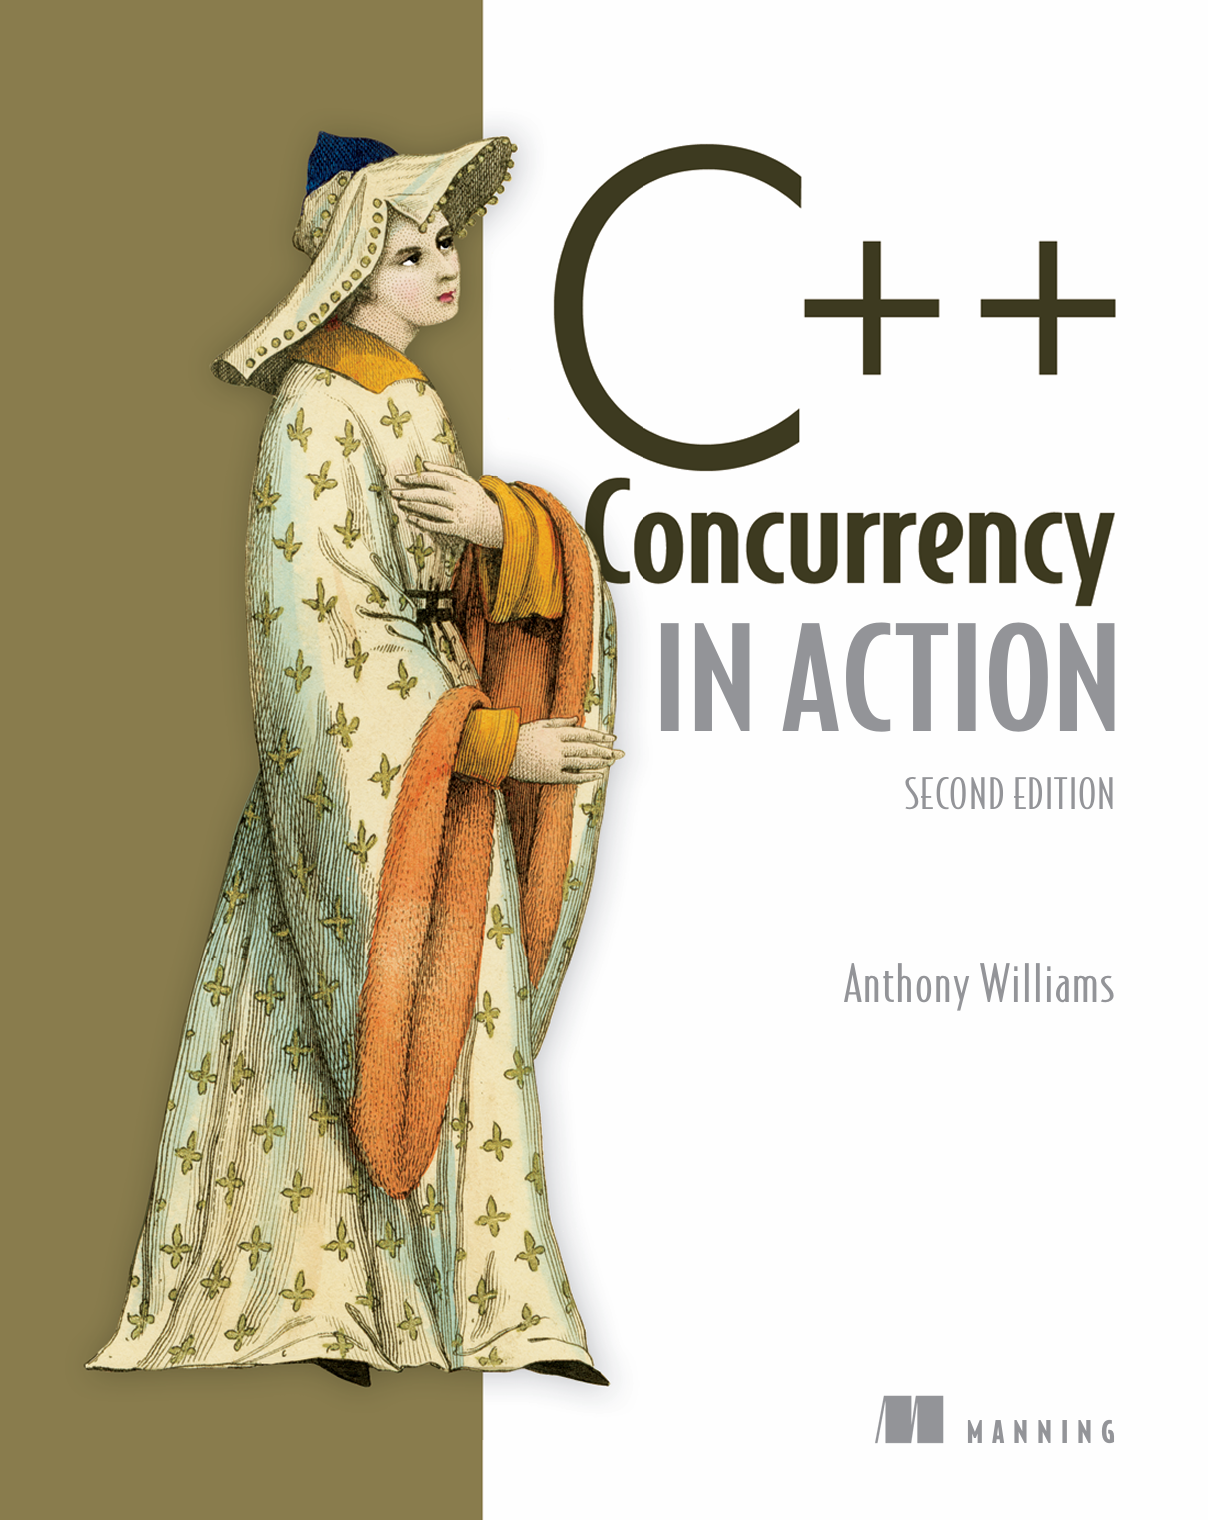
\includegraphics[width=0.8\textwidth]{day8_pm/img/1-book.png}
			\end{center}

		\end{column}
		\begin{column}{0.6\textwidth}
			\begin{itemize}
				\item \textbf{Title}: C++ Concurrency in Action (Second Edition)
				\item \textbf{Authors}: Anthony Williams
				\item \textbf{Publisher}: Manning Publications
			\end{itemize}
		\end{column}
	\end{columns}
\end{frame}

% 本节课的内容大纲
\begin{frame}[fragile]{\emoji{book} Outline}
\section{C++ Quick Start}

\subsection{C++ vs C: Key Differences}
\begin{frame}[fragile]{\emoji{gear} C++ vs C: Core Differences}
	\begin{columns}
		\begin{column}{0.5\textwidth}
			\textbf{C Style}
			\begin{minted}{c}
#include <stdio.h>
#include <stdlib.h>

void print_msg(void) {
    printf("Hello from C!\n");
}

int main() {
    FILE* fp = fopen("test.txt", "r");
    if (fp) {
        // Manual resource management
        fclose(fp);
    }
    return 0;
}
			\end{minted}
		\end{column}
		\begin{column}{0.5\textwidth}
			\textbf{C++ Style}
			\begin{minted}{cpp}
#include <iostream>
#include <fstream>

void print_msg() {
    std::cout << "Hello from C++!" << std::endl;
}

class FileHandler {
public:
    FileHandler(const char* fname)
        : fp(std::fopen(fname, "r")) {}
    ~FileHandler() { if(fp) std::fclose(fp); }
private:
    FILE* fp;
};

int main() {
    FileHandler fh("test.txt");  // RAII
    return 0;
}
			\end{minted}
		\end{column}
	\end{columns}
\end{frame}

\begin{frame}[fragile]{\emoji{link} References vs Pointers}
	\begin{columns}
		\begin{column}{0.5\textwidth}
			\textbf{C Pointers}
			\begin{minted}{c}
void swap_c(int* a, int* b) {
    int temp = *a;
    *a = *b;
    *b = temp;
}

int main() {
    int x = 5, y = 10;
    swap_c(&x, &y);  // Pass addresses
    printf("x=%d, y=%d\n", x, y);
    return 0;
}
			\end{minted}
		\end{column}
		\begin{column}{0.5\textwidth}
			\textbf{C++ References}
			\begin{minted}{cpp}
void swap_cpp(int& a, int& b) {
    int temp = a;
    a = b;
    b = temp;
}

int main() {
    int x = 5, y = 10;
    swap_cpp(x, y);  // Direct pass
    std::cout << "x=" << x << ", y=" << y << std::endl;
    return 0;
}
			\end{minted}
		\end{column}
	\end{columns}

	\vspace{0.5em}
	\textbf{Key Differences:}
	\begin{itemize}
		\item References must be initialized and cannot be reassigned
		\item No pointer arithmetic with references
		\item Cleaner syntax for function parameters
	\end{itemize}
\end{frame}

\subsection{Essential Features for Concurrency}
\begin{frame}[fragile]{\emoji{rocket} Lambda Expressions: The Core of Thread Functions}
	\begin{columns}
		\begin{column}{0.5\textwidth}
			\textbf{C Function Pointers}
			\begin{minted}{c}
#include <pthread.h>

void* thread_func(void* arg) {
    int id = *(int*)arg;
    printf("Thread %d running\n", id);
    return NULL;
}

int main() {
    pthread_t thread;
    int id = 1;
    pthread_create(&thread, NULL,
                   thread_func, &id);
    pthread_join(thread, NULL);
    return 0;
}
			\end{minted}
		\end{column}
		\begin{column}{0.5\textwidth}
			\textbf{C++ Lambda}
			\begin{minted}{cpp}
#include <thread>
#include <iostream>

int main() {
    int id = 1;

    // Lambda expression
    auto thread_func = [id]() {
        std::cout << "Thread " << id
                  << " running" << std::endl;
    };

    std::thread t(thread_func);
    t.join();

    return 0;
}
			\end{minted}
		\end{column}
	\end{columns}

	\vspace{0.5em}
	\textbf{Lambda Capture Modes:}
	\begin{itemize}
		\item \texttt{[]} - Capture nothing
		\item \texttt{[=]} - Capture by value
		\item \texttt{[\&]} - Capture by reference
		\item \texttt{[id]} - Capture specific variable by value
	\end{itemize}
\end{frame}

\begin{frame}[fragile]{\emoji{brain} Auto Type Deduction \& Smart Pointers}
	\begin{columns}
		\begin{column}{0.5\textwidth}
			\textbf{Auto Type Deduction}
			\begin{minted}{cpp}
#include <vector>
#include <map>

int main() {
    auto x = 42;              // int
    auto y = 3.14;            // double
    auto str = "Hello";       // const char*

    std::vector<int> vec{1,2,3};
    auto it = vec.begin();    // vector<int>::iterator

    // Complex types made simple
    std::map<std::string, int> m;
    for(auto& pair : m) {     // Range-based for
        std::cout << pair.first << std::endl;
    }

    return 0;
}
			\end{minted}
		\end{column}
		\begin{column}{0.5\textwidth}
			\textbf{Smart Pointers}
			\begin{minted}{cpp}
#include <memory>

class Resource {
public:
    Resource() { std::cout << "Created\n"; }
    ~Resource() { std::cout << "Destroyed\n"; }
};

int main() {
    // Automatic memory management
    auto ptr = std::make_unique<Resource>();

    // Shared ownership
    auto shared1 = std::make_shared<Resource>();
    auto shared2 = shared1;  // Reference count: 2

    // Automatic cleanup when out of scope
    return 0;
}
			\end{minted}
		\end{column}
	\end{columns}

	\vspace{0.5em}
	\textbf{Benefits:}
	\begin{itemize}
		\item Automatic memory management
		\item Exception safety
		\item Clear ownership semantics
	\end{itemize}
\end{frame}

\section{CPU Parallel Framework Overview}

\subsection{Framework Comparison}
\begin{frame}[fragile]{\emoji{balance-scale} Parallel Programming Framework Comparison}
	\begin{table}[h]
		\centering
		\small
		\begin{tabular}{|l|c|c|c|}
			\hline
			\textbf{Feature}     & \textbf{OpenMP}    & \textbf{MPI}         & \textbf{C++ Thread} \\
			\hline
			Programming Model    & Compiler Directive & Message Passing      & Native API          \\
			Memory Model         & Shared Memory      & Distributed Memory   & Shared Memory       \\
			Learning Curve       & Easy               & Moderate             & Moderate            \\
			Control Granularity  & Coarse             & Fine                 & Very Fine           \\
			Debugging Difficulty & Low                & High                 & High                \\
			\hline
			\textbf{Use Cases}   & Regular Loops      & Cross-node Computing & Complex Task Sched. \\
			                     & Data Parallelism   & Large-scale HPC      & Event-driven Apps   \\
			\hline
		\end{tabular}
	\end{table}

	\vspace{1em}
	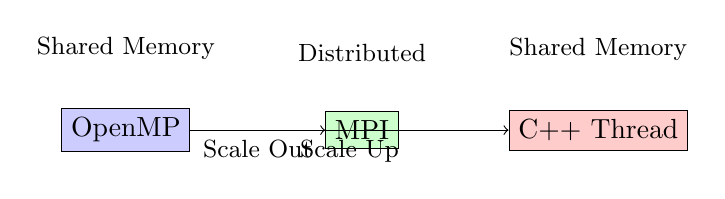
\begin{tikzpicture}
		\node[draw, rectangle, fill=blue!20] (openmp) at (0,0) {OpenMP};
		\node[draw, rectangle, fill=green!20] (mpi) at (3,0) {MPI};
		\node[draw, rectangle, fill=red!20] (cpp) at (6,0) {C++ Thread};

		\node[above] at ([yshift=0.5cm]openmp.north) {\small Shared Memory};
		\node[above] at ([yshift=0.5cm]mpi.north) {\small Distributed};
		\node[above] at ([yshift=0.5cm]cpp.north) {\small Shared Memory};

		\draw[->] (openmp) -- node[midway, below] {\small Scale Up} (cpp);
		\draw[->] (openmp) -- node[midway, below] {\small Scale Out} (mpi);
	\end{tikzpicture}
\end{frame}

\begin{frame}[fragile]{\emoji{gear} When to Use Which Framework?}
	\begin{tikzpicture}[node distance=2cm]
		\node[draw, rectangle, fill=yellow!20] (start) {Parallel Task};

		\node[draw, diamond, fill=blue!10] (memory) at ([yshift=-2cm]start.south) {Data Distribution?};

		\node[draw, rectangle, fill=green!20] (openmp) at ([shift={(-2cm,-2cm)}]memory.south west) {OpenMP};
		\node[draw, rectangle, fill=red!20] (distributed) at ([shift={(2cm,-2cm)}]memory.south east) {Cross-node?};

		\node[draw, rectangle, fill=orange!20] (cpp) at ([shift={(-2cm,-2cm)}]distributed.south west) {C++ Thread};
		\node[draw, rectangle, fill=purple!20] (mpi) at ([shift={(2cm,-2cm)}]distributed.south east) {MPI};

		\draw[->] (start) -- (memory);
		\draw[->] (memory) -- node[left] {Regular Loop} (openmp);
		\draw[->] (memory) -- node[right] {Complex Logic} (distributed);
		\draw[->] (distributed) -- node[left] {Single Node} (cpp);
		\draw[->] (distributed) -- node[right] {Multi-node} (mpi);
	\end{tikzpicture}

	\vspace{1em}
	\textbf{Decision Factors:}
	\begin{itemize}
		\item \textbf{Data locality}: Shared vs distributed memory
		\item \textbf{Task complexity}: Regular patterns vs irregular workloads
		\item \textbf{Scale requirements}: Single node vs cluster
		\item \textbf{Control needs}: Coarse-grained vs fine-grained control
	\end{itemize}
\end{frame}

\subsection{Thread Lifecycle Management}
\begin{frame}[fragile]{\emoji{thread} C++ Thread Basics: Creation and Management}
	\begin{columns}
		\begin{column}{0.5\textwidth}
			\textbf{C pthread Example}
			\begin{minted}[fontsize=\scriptsize]{c}
#include <pthread.h>
#include <stdio.h>

void* worker(void* arg) {
    int id = *(int*)arg;
    printf("Worker %d running\n", id);
    return NULL;
}

int main() {
    pthread_t threads[4];
    int ids[4];

    for(int i = 0; i < 4; i++) {
        ids[i] = i;
        pthread_create(&threads[i], NULL,
                       worker, &ids[i]);
    }

    for(int i = 0; i < 4; i++) {
        pthread_join(threads[i], NULL);
    }

    return 0;
}
			\end{minted}
		\end{column}
		\begin{column}{0.5\textwidth}
			\textbf{C++ std::thread Example}
			\begin{minted}[fontsize=\scriptsize]{cpp}
#include <thread>
#include <vector>
#include <iostream>

void worker(int id) {
    std::cout << "Worker " << id
              << " running" << std::endl;
}

int main() {
    std::vector<std::thread> threads;

    // Create threads
    for(int i = 0; i < 4; i++) {
        threads.emplace_back(worker, i);
    }

    // Wait for completion
    for(auto& t : threads) {
        t.join();
    }

    return 0;
}
			\end{minted}
		\end{column}
	\end{columns}

	\vspace{0.5em}
	\textbf{C++ Advantages:}
	\begin{itemize}
		\item Type-safe parameter passing
		\item RAII automatic resource management
		\item Exception safety
	\end{itemize}
\end{frame}

\begin{frame}[fragile]{\emoji{warning} Parameter Passing Pitfalls}
	\begin{minted}[fontsize=\scriptsize]{cpp}
#include <thread>
#include <iostream>
#include <vector>

void print_value(int val) {
    std::cout << "Value: " << val << std::endl;
}

void increment(int& val) {
    val++;
}

int main() {
    int x = 42;

    // Pass by value - safe
    std::thread t1(print_value, x);

    // This won't compile - can't pass reference directly
    // std::thread t2(increment, x);

    // Correct way to pass reference
    std::thread t2(increment, std::ref(x));

    // Dangerous - reference to local variable
    std::vector<std::thread> threads;
    for(int i = 0; i < 3; i++) {
        // threads.emplace_back(print_value, i);  // Dangerous!
        threads.emplace_back(print_value, i);     // OK - copy
    }

    t1.join();
    t2.join();

    for(auto& t : threads) {
        t.join();
    }

    std::cout << "Final x: " << x << std::endl;
    return 0;
}
	\end{minted}
\end{frame}

\begin{frame}[fragile]{\emoji{laptop} Hands-on: Multi-threaded Array Sum}
	\textbf{Task}: Calculate sum of array using multiple threads

	\begin{minted}[fontsize=\scriptsize]{cpp}
#include <thread>
#include <vector>
#include <numeric>
#include <iostream>

void partial_sum(const std::vector<int>& arr,
                 size_t start, size_t end,
                 long long& result) {
    result = 0;
    for(size_t i = start; i < end; i++) {
        result += arr[i];
    }
}

int main() {
    const size_t SIZE = 1000000;
    std::vector<int> data(SIZE, 1);  // All elements = 1

    const int NUM_THREADS = 4;
    std::vector<std::thread> threads;
    std::vector<long long> partial_results(NUM_THREADS, 0);

    size_t chunk_size = SIZE / NUM_THREADS;

    // Create worker threads
    for(int i = 0; i < NUM_THREADS; i++) {
        size_t start = i * chunk_size;
        size_t end = (i == NUM_THREADS-1) ? SIZE : (i+1) * chunk_size;

        threads.emplace_back(partial_sum, std::cref(data),
                           start, end, std::ref(partial_results[i]));
    }

    // Wait for completion and sum results
    for(auto& t : threads) {
        t.join();
    }

    long long total = std::accumulate(partial_results.begin(),
                                    partial_results.end(), 0LL);

    std::cout << "Total sum: " << total << std::endl;
    return 0;
}
	\end{minted}
\end{frame}

\section{Shared Data Synchronization}

\subsection{Race Conditions}
\begin{frame}[fragile]{\emoji{racing-car} Race Condition Demonstration}
	\textbf{The Problem}: Multiple threads accessing shared data simultaneously

	\begin{minted}[fontsize=\scriptsize]{cpp}
#include <thread>
#include <vector>
#include <iostream>

int counter = 0;  // Shared global variable

void increment_unsafe(int iterations) {
    for(int i = 0; i < iterations; i++) {
        counter++;  // NOT thread-safe!
    }
}

int main() {
    const int NUM_THREADS = 4;
    const int ITERATIONS = 100000;

    std::vector<std::thread> threads;

    // Create threads that increment counter
    for(int i = 0; i < NUM_THREADS; i++) {
        threads.emplace_back(increment_unsafe, ITERATIONS);
    }

    // Wait for all threads to complete
    for(auto& t : threads) {
        t.join();
    }

    std::cout << "Expected: " << NUM_THREADS * ITERATIONS << std::endl;
    std::cout << "Actual:   " << counter << std::endl;
    std::cout << "Lost:     " << (NUM_THREADS * ITERATIONS - counter) << std::endl;

    return 0;
}
	\end{minted}

	\textbf{Expected output}: 400000 \quad \textbf{Typical actual output}: 387234 (varies!)
\end{frame}

\begin{frame}[fragile]{\emoji{microscope} Why Race Conditions Happen}
	\textbf{Assembly Analysis of} \texttt{counter++}:

	\begin{columns}
		\begin{column}{0.5\textwidth}
			\textbf{C++ Code}
			\begin{minted}[fontsize=\scriptsize]{cpp}
counter++;
			\end{minted}

			\vspace{1em}
			\textbf{Assembly (x86-64)}
			\begin{minted}[fontsize=\scriptsize]{asm}
mov    eax, DWORD PTR [counter]
add    eax, 1
mov    DWORD PTR [counter], eax
			\end{minted}
		\end{column}
		\begin{column}{0.5\textwidth}
			\textbf{Thread Interleaving}
			\begin{table}[h]
				\tiny
				\begin{tabular}{|l|l|l|}
					\hline
					\textbf{Thread 1}  & \textbf{Thread 2}  & \textbf{counter} \\
					\hline
					mov eax, [counter] &                    & 0                \\
					(eax = 0)          &                    & 0                \\
					                   & mov eax, [counter] & 0                \\
					                   & (eax = 0)          & 0                \\
					add eax, 1         &                    & 0                \\
					(eax = 1)          &                    & 0                \\
					                   & add eax, 1         & 0                \\
					                   & (eax = 1)          & 0                \\
					mov [counter], eax &                    & 1                \\
					                   & mov [counter], eax & 1                \\
					\hline
				\end{tabular}
			\end{table}

			\textbf{Result}: Both threads read 0, both write 1
			\\Expected: 2, Actual: 1
		\end{column}
	\end{columns}

	\vspace{0.5em}
	\textbf{Critical Section}: The portion of code that accesses shared resources
\end{frame}

\subsection{Mutexes and RAII}
\begin{frame}[fragile]{\emoji{lock} From C Mutexes to C++ RAII Locks}
	\begin{columns}
		\begin{column}{0.5\textwidth}
			\textbf{C pthread Mutex}
			\begin{minted}[fontsize=\scriptsize]{c}
#include <pthread.h>

pthread_mutex_t mutex = PTHREAD_MUTEX_INITIALIZER;
int counter = 0;

void* increment_safe(void* arg) {
    int iterations = *(int*)arg;

    for(int i = 0; i < iterations; i++) {
        pthread_mutex_lock(&mutex);
        counter++;  // Critical section
        pthread_mutex_unlock(&mutex);
    }

    return NULL;
}

// In main: manual cleanup
pthread_mutex_destroy(&mutex);
			\end{minted}
		\end{column}
		\begin{column}{0.5\textwidth}
			\textbf{C++ RAII Lock}
			\begin{minted}[fontsize=\scriptsize]{cpp}
#include <mutex>

std::mutex mtx;
int counter = 0;

void increment_safe(int iterations) {
    for(int i = 0; i < iterations; i++) {
        std::lock_guard<std::mutex> lock(mtx);
        counter++;  // Critical section
        // Automatic unlock when lock goes out of scope
    }
}

// Automatic cleanup - no explicit destroy needed
			\end{minted}
		\end{column}
	\end{columns}

	\vspace{0.5em}
	\textbf{RAII Benefits}:
	\begin{itemize}
		\item \textbf{Exception Safety}: Lock released even if exception thrown
		\item \textbf{No Manual Management}: Automatic acquire/release
		\item \textbf{Scope-based}: Clear lifetime semantics
	\end{itemize}
\end{frame}

\begin{frame}[fragile]{\emoji{hammer-and-wrench} Fixed Counter Example}
	\begin{minted}[fontsize=\scriptsize]{cpp}
#include <thread>
#include <vector>
#include <mutex>
#include <iostream>

std::mutex counter_mutex;
int counter = 0;

void increment_safe(int iterations) {
    for(int i = 0; i < iterations; i++) {
        std::lock_guard<std::mutex> lock(counter_mutex);
        counter++;  // Now thread-safe!
    }
}

int main() {
    const int NUM_THREADS = 4;
    const int ITERATIONS = 100000;

    std::vector<std::thread> threads;

    // Create threads
    for(int i = 0; i < NUM_THREADS; i++) {
        threads.emplace_back(increment_safe, ITERATIONS);
    }

    // Wait for completion
    for(auto& t : threads) {
        t.join();
    }

    std::cout << "Expected: " << NUM_THREADS * ITERATIONS << std::endl;
    std::cout << "Actual:   " << counter << std::endl;
    std::cout << "Success:  " << (counter == NUM_THREADS * ITERATIONS ? "Y" : "N") << std::endl;

    return 0;
}
	\end{minted}

	\textbf{Output}: Expected: 400000, Actual: 400000, Success: Y
\end{frame}

\subsection{Deadlock Prevention}
\begin{frame}[fragile]{\emoji{skull} Deadlock: The Four Horsemen}
	\textbf{Deadlock Conditions} (All must be present):
	\begin{enumerate}
		\item \textbf{Mutual Exclusion}: Resources cannot be shared
		\item \textbf{Hold and Wait}: Process holds resource while waiting for another
		\item \textbf{No Preemption}: Resources cannot be forcibly taken
		\item \textbf{Circular Wait}: Circular chain of waiting processes
	\end{enumerate}

	\vspace{1em}
	\textbf{Classic Deadlock Example}:
	\begin{minted}[fontsize=\scriptsize]{cpp}
std::mutex mutex1, mutex2;

void thread1() {
    std::lock_guard<std::mutex> lock1(mutex1);  // Lock mutex1
    std::this_thread::sleep_for(std::chrono::milliseconds(10));
    std::lock_guard<std::mutex> lock2(mutex2);  // Wait for mutex2 (held by thread2)
    // Do work...
}

void thread2() {
    std::lock_guard<std::mutex> lock2(mutex2);  // Lock mutex2
    std::this_thread::sleep_for(std::chrono::milliseconds(10));
    std::lock_guard<std::mutex> lock1(mutex1);  // Wait for mutex1 (held by thread1)
    // Do work...
}
	\end{minted}

	\emoji{warning} \textbf{Result}: Both threads wait forever!
\end{frame}

\begin{frame}[fragile]{\emoji{shield} Deadlock Prevention Strategies}
	\textbf{Strategy 1: Ordered Locking}
	\begin{minted}[fontsize=\scriptsize]{cpp}
std::mutex mutex1, mutex2;

void thread1() {
    std::lock_guard<std::mutex> lock1(mutex1);  // Always lock in same order
    std::lock_guard<std::mutex> lock2(mutex2);
    // Do work...
}

void thread2() {
    std::lock_guard<std::mutex> lock1(mutex1);  // Same order as thread1
    std::lock_guard<std::mutex> lock2(mutex2);
    // Do work...
}
	\end{minted}

	\textbf{Strategy 2: Atomic Multi-lock}
	\begin{minted}[fontsize=\scriptsize]{cpp}
void thread1() {
    std::unique_lock<std::mutex> lock1(mutex1, std::defer_lock);
    std::unique_lock<std::mutex> lock2(mutex2, std::defer_lock);

    std::lock(lock1, lock2);  // Atomic acquisition of both locks
    // Do work...
}  // Automatic release of both locks

void thread2() {
    std::unique_lock<std::mutex> lock1(mutex1, std::defer_lock);
    std::unique_lock<std::mutex> lock2(mutex2, std::defer_lock);

    std::lock(lock1, lock2);  // Same atomic acquisition
    // Do work...
}
	\end{minted}
\end{frame}

\begin{frame}[fragile]{\emoji{bank} Practical Example: Bank Transfer}
	\begin{minted}[fontsize=\scriptsize]{cpp}
#include <mutex>
#include <iostream>

class BankAccount {
private:
    double balance;
    mutable std::mutex mtx;

public:
    BankAccount(double initial) : balance(initial) {}

    double get_balance() const {
        std::lock_guard<std::mutex> lock(mtx);
        return balance;
    }

    // Safe transfer using ordered locking
    static void transfer(BankAccount& from, BankAccount& to, double amount) {
        // Ensure consistent lock ordering by address
        if (&from < &to) {
            std::lock_guard<std::mutex> lock1(from.mtx);
            std::lock_guard<std::mutex> lock2(to.mtx);
            from.balance -= amount;
            to.balance += amount;
        } else {
            std::lock_guard<std::mutex> lock1(to.mtx);
            std::lock_guard<std::mutex> lock2(from.mtx);
            from.balance -= amount;
            to.balance += amount;
        }
    }
};

int main() {
    BankAccount alice(1000);
    BankAccount bob(500);

    std::thread t1([&]() { BankAccount::transfer(alice, bob, 100); });
    std::thread t2([&]() { BankAccount::transfer(bob, alice, 50); });

    t1.join();
    t2.join();

    std::cout << "Alice: $" << alice.get_balance() << std::endl;
    std::cout << "Bob: $" << bob.get_balance() << std::endl;

    return 0;
}
	\end{minted}
\end{frame}

\section{Producer-Consumer Model}

\subsection{The Need for Condition Variables}
\begin{frame}[fragile]{\emoji{sleeping} Why Not Just Use Busy-Waiting?}
	\textbf{Naive Approach: Polling}
	\begin{minted}[fontsize=\scriptsize]{cpp}
#include <queue>
#include <mutex>
#include <thread>

std::queue<int> buffer;
std::mutex buffer_mutex;
bool done = false;

void consumer_busy_wait() {
    while (!done) {
        std::lock_guard<std::mutex> lock(buffer_mutex);
        if (!buffer.empty()) {
            int item = buffer.front();
            buffer.pop();
            std::cout << "Consumed: " << item << std::endl;
        }
        // Busy waiting - wastes CPU cycles!
    }
}
	\end{minted}

	\vspace{0.5em}
	\textbf{Problems with Busy-Waiting}:
	\begin{itemize}
		\item \emoji{fire} \textbf{CPU Waste}: Constant checking consumes cycles
		\item \emoji{battery} \textbf{Power Drain}: High energy consumption
		\item \emoji{lock} \textbf{Lock Contention}: Frequent mutex acquisition
		\item \emoji{chart-decreasing} \textbf{Poor Scalability}: Performance degrades with more threads
	\end{itemize}

	\vspace{0.5em}
	\emoji{bulb} \textbf{Solution}: Condition Variables - Sleep until notified!
\end{frame}

\subsection{Condition Variables}
\begin{frame}[fragile]{\emoji{bell} Condition Variables: Efficient Waiting}
	\textbf{Core Operations}:
	\begin{itemize}
		\item \texttt{wait(lock, predicate)}: Sleep until condition is true
		\item \texttt{notify\_one()}: Wake up one waiting thread
		\item \texttt{notify\_all()}: Wake up all waiting threads
	\end{itemize}

	\vspace{0.5em}
	\textbf{Basic Pattern}:
	\begin{minted}[fontsize=\scriptsize]{cpp}
#include <condition_variable>
#include <mutex>

std::mutex mtx;
std::condition_variable cv;
bool ready = false;

void waiter() {
    std::unique_lock<std::mutex> lock(mtx);

    // Wait until ready becomes true
    cv.wait(lock, []{ return ready; });

    // Proceed when condition is met
    std::cout << "Condition met, proceeding..." << std::endl;
}

void notifier() {
    {
        std::lock_guard<std::mutex> lock(mtx);
        ready = true;  // Set condition
    }
    cv.notify_one();  // Wake up waiter
}
	\end{minted}

	\emoji{warning} \textbf{Key Points}:
	\begin{itemize}
		\item Always use \texttt{unique\_lock} with condition variables
		\item Always check condition in a loop or use predicate form
		\item Modify shared state before notifying
	\end{itemize}
\end{frame}

\begin{frame}[fragile]{\emoji{gear} How Condition Variables Work}
	\textbf{Internal Mechanism}:

	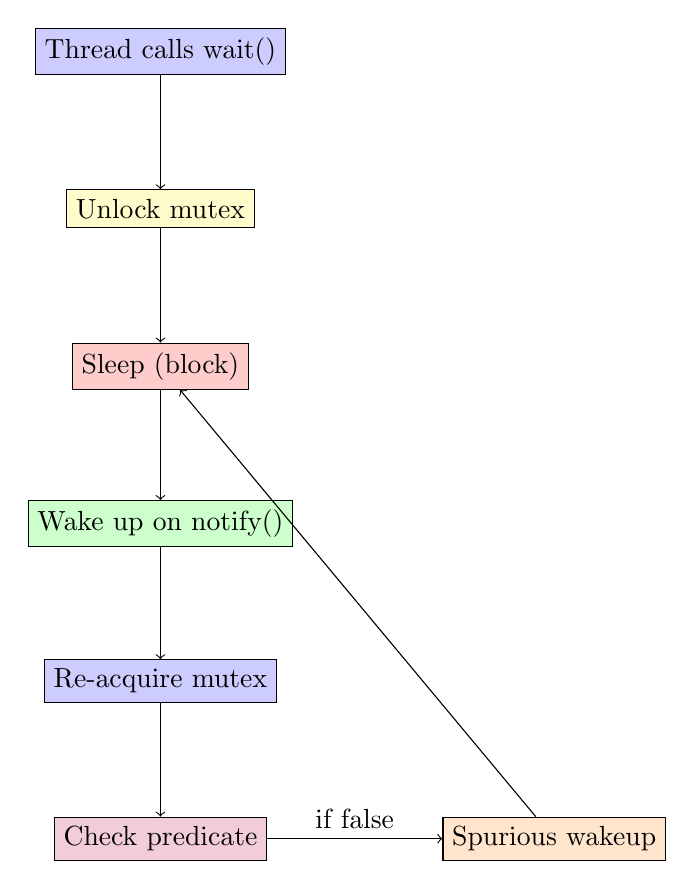
\begin{tikzpicture}[node distance=2cm]
		% Nodes
		\node[draw, rectangle, fill=blue!20] (thread) {Thread calls wait()};
		\node[draw, rectangle, fill=yellow!20, below of=thread] (unlock) {Unlock mutex};
		\node[draw, rectangle, fill=red!20, below of=unlock] (sleep) {Sleep (block)};
		\node[draw, rectangle, fill=green!20, below of=sleep] (wakeup) {Wake up on notify()};
		\node[draw, rectangle, fill=blue!20, below of=wakeup] (relock) {Re-acquire mutex};
		\node[draw, rectangle, fill=purple!20, below of=relock] (check) {Check predicate};
		\node[draw, rectangle, fill=orange!20, right of=check, xshift=3cm] (spurious) {Spurious wakeup};

		% Arrows
		\draw[->] (thread) -- (unlock);
		\draw[->] (unlock) -- (sleep);
		\draw[->] (sleep) -- (wakeup);
		\draw[->] (wakeup) -- (relock);
		\draw[->] (relock) -- (check);
		\draw[->] (check) -- node[above] {if false} (spurious);
		\draw[->] (spurious) -- (sleep);
	\end{tikzpicture}

	\vspace{0.5em}
	\textbf{Why Use Predicates?}
	\begin{minted}[fontsize=\scriptsize]{cpp}
// Vulnerable to spurious wakeups
cv.wait(lock);
if (condition) { /* work */ }

// Robust against spurious wakeups
cv.wait(lock, []{ return condition; });
// Equivalent to:
while (!condition) {
    cv.wait(lock);
}
	\end{minted}
\end{frame}

\subsection{Thread-Safe Queue Implementation}
\begin{frame}[fragile]{\emoji{package} Thread-Safe Queue Design}
	\begin{minted}[fontsize=\scriptsize]{cpp}
#include <queue>
#include <mutex>
#include <condition_variable>

template<typename T>
class ThreadSafeQueue {
private:
    std::queue<T> queue_;
    mutable std::mutex mutex_;
    std::condition_variable condition_;

public:
    void push(const T& item) {
        {
            std::lock_guard<std::mutex> lock(mutex_);
            queue_.push(item);
        }
        condition_.notify_one();  // Notify waiting consumers
    }

    T pop() {
        std::unique_lock<std::mutex> lock(mutex_);

        // Wait until queue is not empty
        condition_.wait(lock, [this] { return !queue_.empty(); });

        T item = queue_.front();
        queue_.pop();
        return item;
    }

    bool empty() const {
        std::lock_guard<std::mutex> lock(mutex_);
        return queue_.empty();
    }

    size_t size() const {
        std::lock_guard<std::mutex> lock(mutex_);
        return queue_.size();
    }
};
	\end{minted}
\end{frame}

\subsection{Producer-Consumer Implementation}
\begin{frame}[fragile]{\emoji{factory} Complete Producer-Consumer Example}
\begin{minted}[fontsize=\scriptsize]{cpp}
#include <iostream>
#include <thread>
#include <chrono>
#include <random>

ThreadSafeQueue<int> shared_queue;
bool production_done = false;
std::mutex done_mutex;

void producer(int id, int num_items) {
    std::random_device rd;
    std::mt19937 gen(rd());
    std::uniform_int_distribution<> dis(1, 100);

    for (int i = 0; i < num_items; ++i) {
        int item = dis(gen);
        shared_queue.push(item);

        std::cout << "Producer " << id << " produced: " << item << std::endl;

        // Simulate production time
        std::this_thread::sleep_for(std::chrono::milliseconds(100));
    }

    std::cout << "Producer " << id << " finished" << std::endl;
}

void consumer(int id) {
    while (true) {
        // Check if production is done and queue is empty
        {
            std::lock_guard<std::mutex> lock(done_mutex);
            if (production_done && shared_queue.empty()) {
                break;
            }
        }

        try {
            int item = shared_queue.pop();
            std::cout << "Consumer " << id << " consumed: " << item << std::endl;

            // Simulate consumption time
            std::this_thread::sleep_for(std::chrono::milliseconds(150));
        } catch (...) {
            // Handle empty queue case if needed
        }
    }

    std::cout << "Consumer " << id << " finished" << std::endl;
}
	\end{minted}
\end{frame}

\begin{frame}[fragile]{\emoji{rocket} Running the Producer-Consumer System}
	\begin{minted}[fontsize=\scriptsize]{cpp}
int main() {
    const int NUM_PRODUCERS = 2;
    const int NUM_CONSUMERS = 3;
    const int ITEMS_PER_PRODUCER = 5;

    std::vector<std::thread> producers;
    std::vector<std::thread> consumers;

    // Start consumers first
    for (int i = 0; i < NUM_CONSUMERS; ++i) {
        consumers.emplace_back(consumer, i);
    }

    // Start producers
    for (int i = 0; i < NUM_PRODUCERS; ++i) {
        producers.emplace_back(producer, i, ITEMS_PER_PRODUCER);
    }

    // Wait for all producers to finish
    for (auto& p : producers) {
        p.join();
    }

    // Signal that production is done
    {
        std::lock_guard<std::mutex> lock(done_mutex);
        production_done = true;
    }

    // Wait for all consumers to finish
    for (auto& c : consumers) {
        c.join();
    }

    std::cout << "All threads completed successfully!" << std::endl;

    return 0;
}
	\end{minted}

	\textbf{Expected Behavior}:
	\begin{itemize}
		\item Producers generate items at different rates
		\item Consumers process items as they become available
		\item No race conditions or data corruption
		\item Graceful shutdown when production completes
	\end{itemize}
\end{frame}

\begin{frame}[fragile]{\emoji{chart-increasing} Performance Comparison}
	\textbf{Busy-Waiting vs Condition Variables}

	\begin{table}[h]
		\centering
		\begin{tabular}{|l|c|c|}
			\hline
			\textbf{Metric}   & \textbf{Busy-Waiting} & \textbf{Condition Variables} \\
			\hline
			CPU Usage         & 95-100\%              & 5-15\%                       \\
			Response Time     & Low                   & Low                          \\
			Throughput        & Medium                & High                         \\
			Power Consumption & High                  & Low                          \\
			Scalability       & Poor                  & Good                         \\
			\hline
		\end{tabular}
	\end{table}

	\vspace{1em}
	\textbf{Real-world Applications}:
	\begin{itemize}
		\item \textbf{Web Servers}: Request queue processing
		\item \textbf{Database Systems}: Transaction queue management
		\item \textbf{Game Engines}: Event processing pipelines
		\item \textbf{Media Players}: Audio/video buffer management
	\end{itemize}
\end{frame}

\section{Summary and Framework Selection}

\subsection{Core Concepts Review}
\begin{frame}[fragile]{\emoji{brain} C++ Concurrency Core Concepts}
	\textbf{The Three Pillars}:

	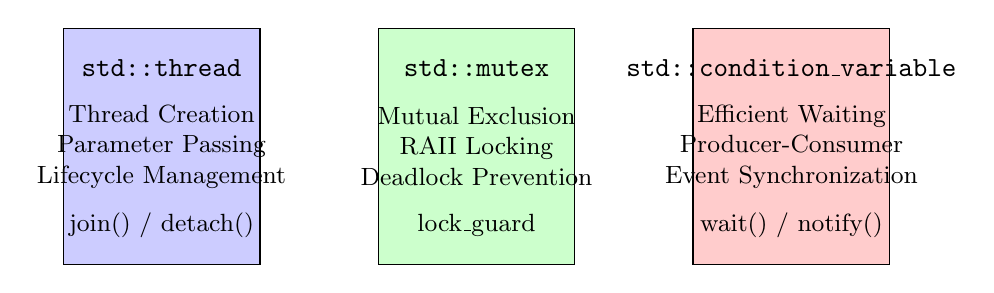
\begin{tikzpicture}
		% Pillar 1: Thread
		\node[draw, rectangle, fill=blue!20, minimum height=3cm, minimum width=2.5cm] (thread) at (0,0) {};
		\node[font=\bfseries] at (0,1) {\texttt{std::thread}};
		\node[font=\small, align=center] at (0,0) {Thread Creation\\Parameter Passing\\Lifecycle Management};
		\node[font=\small] at (0,-1) {join() / detach()};

		% Pillar 2: Mutex
		\node[draw, rectangle, fill=green!20, minimum height=3cm, minimum width=2.5cm] (mutex) at (4,0) {};
		\node[font=\bfseries] at (4,1) {\texttt{std::mutex}};
		\node[font=\small, align=center] at (4,0) {Mutual Exclusion\\RAII Locking\\Deadlock Prevention};
		\node[font=\small] at (4,-1) {lock\_guard};

		% Pillar 3: Condition Variable
		\node[draw, rectangle, fill=red!20, minimum height=3cm, minimum width=2.5cm] (cv) at (8,0) {};
		\node[font=\bfseries] at (8,1) {\texttt{std::condition\_variable}};
		\node[font=\small, align=center] at (8,0) {Efficient Waiting\\Producer-Consumer\\Event Synchronization};
		\node[font=\small] at (8,-1) {wait() / notify()};
	\end{tikzpicture}

	\vspace{2em}
	\textbf{Best Practices Checklist}:
	\begin{itemize}
		\item \emoji{check-mark} Always join() or detach() threads
		\item \emoji{check-mark} Use RAII locks (\texttt{lock\_guard}, \texttt{unique\_lock})
		\item \emoji{check-mark} Avoid deadlocks with ordered locking
		\item \emoji{check-mark} Use condition variables instead of busy-waiting
		\item \emoji{check-mark} Pass by value or \texttt{std::ref} explicitly
	\end{itemize}
\end{frame}

\subsection{Framework Selection Guide}
\begin{frame}[fragile]{\emoji{compass} When to Choose Which Framework}
	\begin{tikzpicture}[node distance=1.5cm]
		% Decision tree
		\node[draw, diamond, fill=yellow!20] (start) {Parallel Task};

		\node[draw, diamond, below left of=start, fill=blue!10] (pattern) {Regular Pattern?};
		\node[draw, diamond, below right of=start, fill=blue!10] (scale) {Scale Requirement?};

		\node[draw, rectangle, below of=pattern, fill=green!20] (openmp) {OpenMP};
		\node[draw, rectangle, below left of=scale, fill=red!20] (cpp) {C++ Thread};
		\node[draw, rectangle, below right of=scale, fill=purple!20] (mpi) {MPI};

		% Arrows with labels
		\draw[->] (start) -- node[above left] {Data Parallel} (pattern);
		\draw[->] (start) -- node[above right] {Task Parallel} (scale);
		\draw[->] (pattern) -- node[left] {Yes} (openmp);
		\draw[->] (scale) -- node[above left] {Single Node} (cpp);
		\draw[->] (scale) -- node[above right] {Multi-node} (mpi);
	\end{tikzpicture}

	\vspace{1em}
	\textbf{Detailed Comparison}:
	\begin{table}[h]
		\centering
		\tiny
		\begin{tabular}{|l|c|c|c|}
			\hline
			\textbf{Criteria}    & \textbf{OpenMP} & \textbf{C++ Thread} & \textbf{MPI} \\
			\hline
			Learning Curve       & Easy            & Moderate            & Hard         \\
			Development Time     & Fast            & Medium              & Slow         \\
			Performance Control  & Low             & High                & High         \\
			Debugging Complexity & Low             & Medium              & High         \\
			Memory Model         & Shared          & Shared              & Distributed  \\
			Scalability          & 1-64 cores      & 1-32 cores          & 1000s cores  \\
			\hline
			\textbf{Best For}    & Loops           & Complex Logic       & HPC Clusters \\
			\hline
		\end{tabular}
	\end{table}
\end{frame}

\subsection{Comprehensive Example}
\begin{frame}[fragile]{\emoji{dart} Monte Carlo π Calculation: All Frameworks}
	\textbf{Problem}: Estimate π using random point sampling

	\begin{columns}
		\begin{column}{0.3\textwidth}
			\textbf{OpenMP Version}
			\begin{minted}{cpp}
#include <omp.h>
#include <random>

double monte_carlo_openmp(long samples) {
    long count = 0;

    #pragma omp parallel reduction(+:count)
    {
        std::random_device rd;
        std::mt19937 gen(rd());
        std::uniform_real_distribution<> dis(0.0, 1.0);

        #pragma omp for
        for(long i = 0; i < samples; i++) {
            double x = dis(gen);
            double y = dis(gen);
            if(x*x + y*y <= 1.0) {
                count++;
            }
        }
    }

    return 4.0 * count / samples;
}
			\end{minted}
		\end{column}
		\begin{column}{0.35\textwidth}
			\textbf{C++ Thread Version}
			\begin{minted}{cpp}
#include <thread>
#include <vector>
#include <atomic>

std::atomic<long> global_count(0);

void worker(long samples) {
    std::random_device rd;
    std::mt19937 gen(rd());
    std::uniform_real_distribution<> dis(0.0, 1.0);

    long local_count = 0;
    for(long i = 0; i < samples; i++) {
        double x = dis(gen);
        double y = dis(gen);
        if(x*x + y*y <= 1.0) {
            local_count++;
        }
    }

    global_count += local_count;
}

double monte_carlo_cpp(long samples) {
    const int num_threads = std::thread::hardware_concurrency();
    std::vector<std::thread> threads;

    long samples_per_thread = samples / num_threads;

    for(int i = 0; i < num_threads; i++) {
        threads.emplace_back(worker, samples_per_thread);
    }

    for(auto& t : threads) {
        t.join();
    }

    return 4.0 * global_count / samples;
}
			\end{minted}
		\end{column}
		\begin{column}{0.35\textwidth}
			\textbf{MPI Version}
			\begin{minted}{cpp}
#include <mpi.h>

double monte_carlo_mpi(long samples) {
    int rank, size;
    MPI_Comm_rank(MPI_COMM_WORLD, &rank);
    MPI_Comm_size(MPI_COMM_WORLD, &size);

    long local_samples = samples / size;
    long local_count = 0;

    std::random_device rd;
    std::mt19937 gen(rd() + rank);
    std::uniform_real_distribution<> dis(0.0, 1.0);

    for(long i = 0; i < local_samples; i++) {
        double x = dis(gen);
        double y = dis(gen);
        if(x*x + y*y <= 1.0) {
            local_count++;
        }
    }

    long global_count;
    MPI_Reduce(&local_count, &global_count, 1,
               MPI_LONG, MPI_SUM, 0, MPI_COMM_WORLD);

    if(rank == 0) {
        return 4.0 * global_count / samples;
    }
    return 0.0;
}
			\end{minted}
		\end{column}
	\end{columns}
\end{frame}

\begin{frame}[fragile]{\emoji{bar-chart} Performance Analysis}
	\textbf{Benchmark Results} (1 billion samples):

	\begin{table}[h]
		\centering
		\begin{tabular}{|l|c|c|c|c|}
			\hline
			\textbf{Framework} & \textbf{Time (s)} & \textbf{Speedup} & \textbf{Accuracy} & \textbf{LOC} \\
			\hline
			Sequential         & 12.5              & 1.0×             & π ≈ 3.141592      & 15           \\
			OpenMP             & 1.8               & 6.9×             & π ≈ 3.141591      & 20           \\
			C++ Thread         & 1.9               & 6.6×             & π ≈ 3.141593      & 35           \\
			MPI (8 nodes)      & 0.3               & 41.7×            & π ≈ 3.141590      & 40           \\
			\hline
		\end{tabular}
	\end{table}

	\vspace{1em}
	\textbf{Trade-offs Analysis}:
	\begin{itemize}
		\item \textbf{OpenMP}: Best effort/performance ratio for shared memory
		\item \textbf{C++ Thread}: Maximum control, good for complex algorithms
		\item \textbf{MPI}: Unmatched scalability for distributed computing
	\end{itemize}

	\vspace{0.5em}
	\textbf{Development Productivity}:
	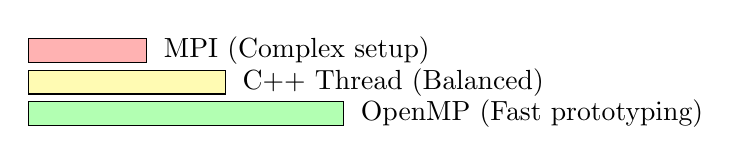
\begin{tikzpicture}
		\draw[fill=green!30] (0,0) rectangle (4,0.3);
		\draw[fill=yellow!30] (0,0.4) rectangle (2.5,0.7);
		\draw[fill=red!30] (0,0.8) rectangle (1.5,1.1);

		\node[right] at (4.1,0.15) {OpenMP (Fast prototyping)};
		\node[right] at (2.6,0.55) {C++ Thread (Balanced)};
		\node[right] at (1.6,0.95) {MPI (Complex setup)};
	\end{tikzpicture}
\end{frame}

\subsection{Advanced Topics Preview}
\begin{frame}[fragile]{\emoji{telescope} Beyond the Basics: Advanced Concurrency}
	\textbf{Topics for Further Exploration}:

	\begin{columns}
		\begin{column}{0.5\textwidth}
			\textbf{Asynchronous Programming}
			\begin{minted}{cpp}
#include <future>

auto future = std::async(std::launch::async,
    []() {
        return expensive_computation();
    });

// Do other work...
auto result = future.get();  // Wait for result
			\end{minted}

			\textbf{Atomic Operations}
			\begin{minted}{cpp}
#include <atomic>

std::atomic<int> counter{0};

void increment() {
    counter.fetch_add(1, std::memory_order_relaxed);
}
			\end{minted}
		\end{column}
		\begin{column}{0.5\textwidth}
			\textbf{Thread Pools}
			\begin{minted}{cpp}
class ThreadPool {
    std::vector<std::thread> workers;
    std::queue<std::function<void()>> tasks;
    std::mutex queue_mutex;
    std::condition_variable condition;

public:
    template<class F>
    void enqueue(F&& f) {
        {
            std::lock_guard<std::mutex> lock(queue_mutex);
            tasks.emplace(std::forward<F>(f));
        }
        condition.notify_one();
    }
};
			\end{minted}
		\end{column}
	\end{columns}

	\vspace{1em}
	\textbf{Learning Path}:
	\begin{enumerate}
		\item Master the basics: \texttt{thread}, \texttt{mutex}, \texttt{condition\_variable}
		\item Explore \texttt{std::async} and \texttt{std::future}
		\item Study atomic operations and memory models
		\item Implement lock-free data structures
		\item Build thread pools and work-stealing algorithms
	\end{enumerate}
\end{frame}


\begin{frame}[fragile]{Takeaways}
	\emoji{star} Important concepts that you should remember today:
	\begin{itemize}
		\item \textbf{C++ Concurrency Trinity}: \texttt{std::thread}, \texttt{std::mutex}, \texttt{std::condition\_variable}
		\item \textbf{RAII Principle}: Automatic resource management with lock guards
		\item \textbf{Producer-Consumer Pattern}: Efficient thread communication
		\item \textbf{Framework Selection}: Choose the right tool for the right job
	\end{itemize}
\end{frame}

% Q&A
\begin{frame}[standout]
	\Huge\textsc{Thank You}

	\vfill

	\LARGE\textsc{Any Questions?}
\end{frame}

\end{document}
